\documentclass[12pt]{extarticle}
\usepackage[utf8]{inputenc}
\usepackage[T1]{fontenc}
\usepackage[english]{babel}
\usepackage{natbib}
\usepackage{gensymb}
\usepackage{graphicx}
\graphicspath{ {./images/} }
\bibliographystyle{apa}

%%%%%%%%%%%%%%%%%%%%%%%%%%%%%%%%%
%Delimitation of the project and working title for the thesis.
%Theoretical hypothesis and/or research question.
%Aim, value and expected impact of the project.
%Scope and timeplan of the project.
%References and materials, the student‘s status of relevant knowledge
%Research method, data collection and analysis, scope and timeframe.
%uggested table of contents for the thesis.%

\title{Parental Effects on Development and Behavior in Threespine Stickleback \textit{Gasterosteus aculeatus} of Lake M\'yvatn, Iceland}
\author{Spencer Edwards, Roll No.}
\date{April 2021}

\begin{document}

\maketitle

\section*{Research Question}
Major questions I want to address:
\begin{itemize}
 \item To what extent are the phenotypes of lake M\'yvatn stickleback 
shaped by maternal and paternal (parental) effects?
 \item Specifically, how much variation in stickleback phenotypes of morphology (For example:  shape, feeding structures), phenology (growth rate, size,  and behavior (For example: feeding behavior, antipredator behavior, shyness/boldness, shoaling) are driven by genetic inheritence vs environmental inheritence?
\end{itemize}

\section*{Relevant Background}
An organism’s phenotype determines its  
Development and early life history are crucial steps for organisms. Consequentially, the traits gained by an organism from its parents during this time are key to its success as an individual.  It is not surprising then, that parental effects, both maternal and paternal, have a major impact on organisms \citep{charmantier_garant_kruuk_2014, Danchin2011, Badyaev2009}. Parental effects, defined as a change in an Offspring's phenotype due to the genotype and/or environment of one or more of its parents, were for a long time considered a nuisance, a deviation from pure heritable traits. Now however we have seen a resurgence of interest in these effects \citep{charmantier_garant_kruuk_2014}. While much research has been done concerning the impact of parental effects on development \citep{Tigreros2021} and behavior of invertebrates (particularly beetles), comparitively less is known about parental effects on vertebrates. Work on teleosts has revealed strong links between parental effects on the co-evolution of behavior and cellular function \citep{Yoshizawa2012}. The connection between parental affects influencing behavior and gene expression has serious implications for evolutionary ecology, because rapid environmental could act as a mechanism for rapid evolution via parental programming of offspring phenotypes, effectively providing their offspring with a ``jump start'' of sorts \citep{Danchin2011, Donelson2018}. 
From the standpoint of quantitative genetics, the phenotype (\textit{P}) is equal to the influence of genes (\textit{G}) and environment (\textit{E}) such that $$P = G + E $$

However, genetic effects from parents can be further broken down into inheritance from genes directly ($I_G$) and inheritance from the parental environment ($I_E$) such that $$P = (I_G + I_E) + G \times E$$

Quantitative genetics uses the relationships between relatives to analyze sources of phenotypic variation, in particular the phenotypic variation caused by complex traits.
The benefit of using a quantitative genetics model is that we can make predictions about where traits come from and test them using a Generalized Linear Mixed Model (GLMM) \citep{Wilson2010, Bolker2009, VanDooren2016}. GLMMs allow us to estimate how much of the phenotype is derived from genetics by breaking down the variance of the phenotype into multiple sources. By portioning the phenotypic variance into genetic and environmental effects (Sometimes referred to as Additive and Residual, respectively), we can extend our analysis to multiple co-varying traits and analyze where multiple traits which are responsible for differences in life-history strategies come from. From there, we can make predictions about how phenotypes will evolve. This is important for managment decisions in an era of rapid global climate change \citep{VanDooren2016}.

Parental effects are of particular interest to evolutionary ecologists because they have the ability to both promote rapid phenotypic diversification and intergration, as well as prevent it through matching develpmental gene expression and timing \citep{Badyaev2009}. When quantifying parental effects, we first need to estiblish if parental effects are expressed, and if so, where in the life-history of the organism they are expressed. From there

Here in Iceland, work on various populations of \textit{Gasterosteus aculeatus} has focused on phenotypic diversity, including phenotypic plasticity \citep{Kristjansson2002, Millet2013}. However, the extent to which parental effects shape the morphology and behavior of lake M\'yvatn stickleback has yet to be investigated. Previous work on different stickleback populations have discovered a range of parental effects, both maternal and paternal. \citet{Bell2018} investigated the heritability of parental behavior (Specifically, fanning of eggs) by male stickleback and found strong heritability of the trait. Furthermore, they concluded that a strong amount of genetic variation could lead the evolvability of the fanning trait. Offspring of male stickleback that experience predation risk have shown to grow smaller and spend less time in the open \citep{Bell2016, Stein2014} Female stickleback have also been shown to pass on phenotypic information to their eggs. An RNAseq study analyzing female stickleback found that eggs from mothers exposed to predators had faster development times, as well as major epigenetic changes and alterations to non-coding genes during development \citep{Mommer2014, Bell2016}.  \\

Another more comprehensive way to quantify parental effects is the breeder's equation. In its simplest form, the breeder's equation includes  \\



%Danchin2011 discusses some evidence for non-genetic inheritence mechanisms and calls for a new extended synthesis %
%rasanen et al consider evidence that maternal effects are not entriely environmental but that the environment does play a cruicial role in determining the impact of these affects, and lays out evidence and examples on an ecological time scale



\section*{Methods}

I will use a half-sibling common garden experiment to assess parental effects in Mývatn stickleback. Stickleback will be collected from Grímsstaðir. Sticklebacks from both shores will then be crossed using standard methods laid out by Schluter. Half-sibling split clutch designs have been used previously to examine the effects of indirect fitness in parasite resistance, as well as transgenerational plasticity in response to temperature in marine stickleback (Barber et al. 2001; Ramler et al. 2014). One of the major problems when considering historical work on parental effects is disentangling genetic and environmental effects (Donelson et al. 2018). Using a Linear Mixed Model (LMM) approach to decompile the effects should be effective. 16 males and 16 breeding females will be collected from the shore of lake M\'yvatn at Grímsstaðir station. Sperm from each male will be split and used to fertilize two females, and eggs from each female will be fertilized by two males. Each family will be split between two tanks to account for tank effects on individuals. A total of 64 tanks will be used to house the 32 full-sib families. Fish will be raised in 10L tanks in a common garden at 13 °C and fed a mixed diet of blood worms (twice a day Tues and Thurs) and pellets (once a day, Mon, Wed, Fri). Fish will be weighed/measured every 3 months until fully grown, when their behavior will be assessed.

\begin{figure}
\centering
 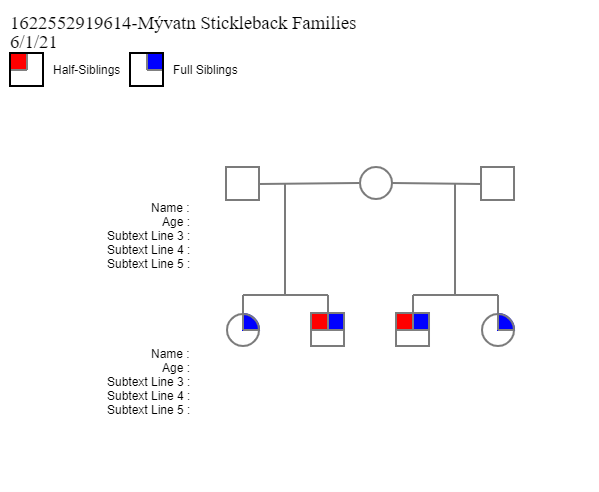
\includegraphics[width=0.7\textwidth]{pedigree}
 \caption{Example pedigree of half-sibling cross}
  \label{fig:pedigree1}
\end{figure}


Proposed Guides: Dr. Bjarni Kristj\'ansson, Department of Aquaculture and Fish Biology, H\'olar University College.
\bibliography{mainbib}

\end{document}

